\chapter{Experiments and Results}
\label{chap:experiments}
This chapter presents a series of experiments designed to answer the research questions posed in \autoref{chap:intro}, focusing on the evaluation of the Mamba-\acrshort{s6} (\acrshort{vms}) model for temporal event spotting in football video. The accuracy and runtime are compared against the \acrshort{tdeed} baseline, I investigate the impact of feature dimensionality, and perform a Bayesian hyperparameter sweep to optimize performance.


\section{Experiment 1: Compare accuracy between \acrshort{tdeed} and mamba}
\label{sec:experiment1}
The first experiment compares accuracy from \acrfull{tdeed} and \acrfull{vms}. The goal is to determine if the \acrshort{vms} model can achieve similar or better accuracy than the \acrshort{tdeed} model. The models are trained on the SoccerNet-V2 dataset \cite{deliege_soccernet-v2_dataset_2021}. They are evaluated using mean average precision (\acrshort{map}) and \acrshort{map}@50 metrics.

\subsection{Setup}
\label{ssec:ex1_setup}
We trained three models on the SoccerNet-V2 dataset \cite{deliege_soccernet-v2_dataset_2021}:  
\begin{itemize}
    \item \acrshort{vms}-80\_20 using an 80\%/20\% train/val split,  
    \item \acrshort{vms}-70\_30 using a 70\%/30\% split, and  
    \item \acrshort{tdeed} with four matches for training and one for validation (equivalent to 80\%/20\%).  
\end{itemize}

All models used default hyperparameters from their original papers. Performance was measured by mean \acrfull{map} and \acrshort{map}@50 under a \(\pm 1\) s tolerance window.

\todo{talk about annotation edit? mentioned in method}

\subsection{Results}
\label{ssec:ex1_results}
\begin{table}[ht]
    \centering
    \begin{tabular}{lccc}
        \toprule
        Model & average \acrshort{map} (\%)  & validation \acrshort{map}@50 (\%) & test \acrshort{map}@50 (\%)\\
        \midrule
        \acrshort{tdeed} &  \textemdash & 20.78 & \textbf{47.65}\\
        \acrshort{vms} (Mamba-\acrshort{s6})   &  \textbf{45.99}   & 43.62 & \textemdash \\
        % \acrshort{vms}-70\_30 (Mamba-\acrshort{s6})   & 48.73 & 46.46 \\
        \bottomrule
    \end{tabular}
    \caption{Accuracy comparison on SoccerNet-V2.}
    \label{tab:results_ex1}
\end{table}

The \acrshort{vms} model (Mamba-\acrshort{s6}) had an average \acrshort{map}, achieving \textbf{45.99\%}. The \acrshort{tdeed} model's average \acrshort{map} is not calculated as there is no \acrshort{iou}, but its validation \acrshort{map}@50 was 20.78\%. In the validation \acrshort{map}@50 category, the \acrshort{vms} model significantly outperformed \acrshort{tdeed}, scoring (43.62\%) compared to \acrshort{tdeed}'s (20.78\%).

Conversely, the \acrshort{tdeed} model achieved a higher test \acrshort{map}@50 of \textbf{47.65\%}. Whereas the corresponding test metric for the \acrshort{vms} model is not provided or calculated. There is a significant disparity between \acrshort{tdeed}'s validation and test performance. This is primarily due to differences in stride during prediction, with the validation model using a stride of two, effectively halving its temporal resolution compared to the test evaluation. 


\subsection{Discussion}
\label{ssec:ex1_discussion}

The large difference in validation \acrshort{map}@50 for \acrshort{tdeed} could be a result of lacking postprocessing. \acrshort{tdeed} uses two different functions for predicting the test \acrshort{map} and the validation \acrshort{map}. The test evaluator applies soft non-maximum suppression to remove redundant detections, while the validation does not remove redundant predictions. In addition to this, the validation predicts with a stride of \(2\), but the test has a stride of \(1\). With \(fps=25\) and a \(tolerance = \pm 1s\), this reduction in temporal resolution hinders the predictions from hitting the tolerance window. 



The \acrshort{vms} model employs a form of post-processing. \acrshort{vms} does little preprocessing, and its only configurable parameter was the top (k) classes to predict in each step. \acrshort{vms} predicts the likelihood of different action classes being present anywhere in the entire video. 

This "top (k)" mechanism, which uses video-level classification scores to refine predictions for temporal segments, is a post-processing technique. It helps in reducing class confusion and boosting correct class assignments by leveraging global video context. \autoref{fig:topk} shows that the baseline with \(topk=2\) and the run with \(topk=12\) behaved quite similarly. The baseline with \(topk=12\) is the same as in \autoref{tab:results_ex1}, while a run with \(topk=2\) achieved 45.85\% average \acrshort{map}.

However, this type of post-processing is different from the "significant postprocessing" (specifically Soft Non-Maximum Suppression - SNMS) that the \acrshort{tdeed} model uses for its test evaluation. SNMS primarily addresses the issue of removing redundant or overlapping detections.

The performance of the \acrshort{vms} model could likely be enhanced by incorporating techniques similar to \acrshort{tdeed}'s test-time post-processing, specifically NMS or SNMS.

The current "top (k)" post-processing in \acrshort{vms} refines the classification and scoring of proposed segments.
NMS/SNMS would address a different aspect: filtering out redundant temporal detections.
These two types of post-processing are not mutually exclusive and can be complementary. Applying NMS/SNMS after the "top (k)" refinement could potentially lead to a further increase in \acrshort{vms}'s \acrshort{map} scores. Particularly for metrics like \acrshort{map}@50, where precise, non-redundant detections are crucial. This would make its evaluation more directly comparable to \acrshort{tdeed}'s test performance.

\begin{figure}
    \centering
    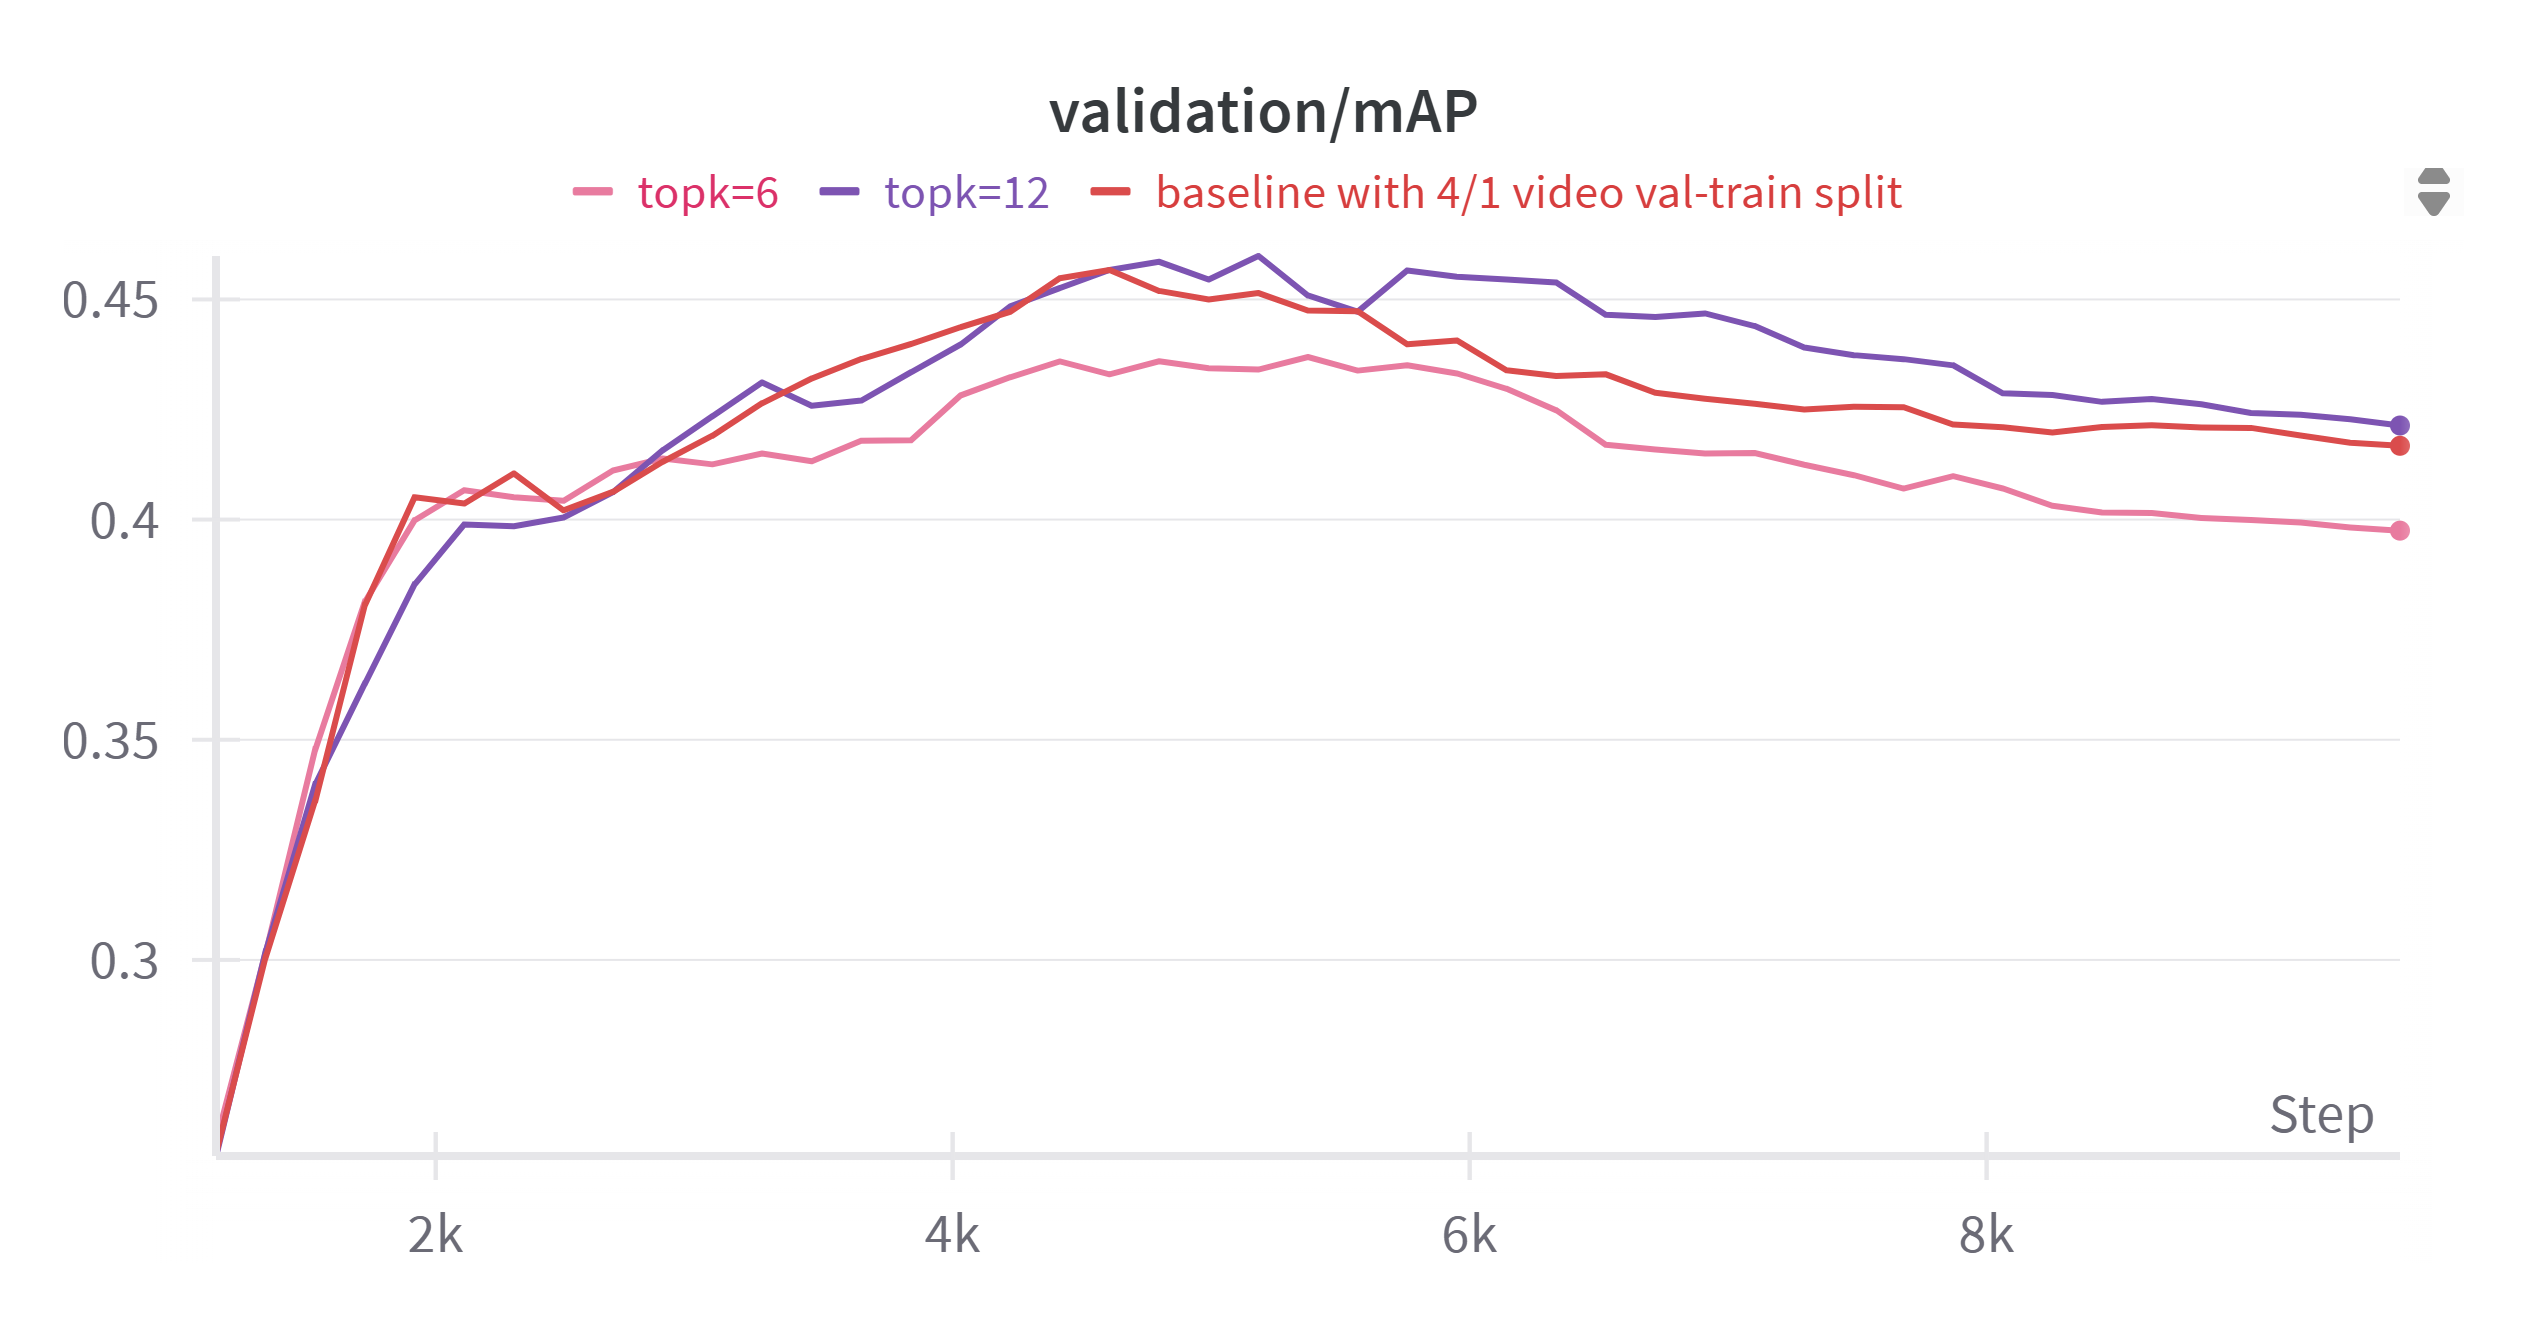
\includegraphics[width=0.75\linewidth]{figures/topk_classes.png}
    \caption{Results from different post-processing top \(k\) classes.}
    \label{fig:topk}
\end{figure}

Using a shorter stride for validation is a technique to increase training speed. In the case of the \acrshort{tdeed} implemented for SoccerNet, the testing phase is weighted more heavily than validation, as it is the submission to a challenge. This is an oversight; a run with \(STRIDE=1\) was run, but not completed in time for discussion. This oversight could be a hindrance to the direct comparison between the validation scores.\improvement{a run with stride=1 is run, but when will it complete? Late according to squeue --start --me}


The temporal discriminability enhancer part of the \acrfull{tdeed} has specialized strategies and components designed to:
\begin{itemize}
    \item improve the distinction between similar actions
    \item improve token discrimination
    \item per frame predictions
\end{itemize}

The focus on enhancing temporal distinctions is one of the keys to success in tasks where small variations in timing or appearance can result in different categories. 

In contrast, Mamba's design captures long-range contexts and provides a broader understanding of the whole video. It is also meant to learn quicker with linear complexity and require less data. It is my theory that with a stronger post-processing pipeline, the \acrshort{map} advantage would be larger. 

The validation set size of a single football game can be problematic. Football games can vary significantly due to teams, play styles, event frequency, and referee threshold for giving fouls, to name a few. There is a risk of bias from the distribution of actions within the validation game. If the validation game is "easy" or "hard", that would severely influence the validation score. A split of 80\% to 20\% validates on one game and trains on four in total. But when the game is split into 90 sections, which are randomly assigned to each category, the validation set is more robust. The result will be more transferable and generalizable. 

\acrshort{vms} runs on any \acrshort{gpu}, but \acrshort{tdeed} needs a lot of memory and only runs on premium GPUs. If computational resources (especially GPU memory and type) are a limiting factor, \acrshort{vms} is the more practical choice. \acrshort{vms} has a simpler post-processing and a clearer GitHub explaining installation steps, which could be more straightforward to deploy. However, without obvious comparisons, it is hard to pick out clear advantages of one model over the other. 

The most significant limitation is the absence of the test \acrshort{map}@50 score for the \acrshort{vms} model. This prevents a direct and complete comparison with \acrshort{tdeed} on this crucial metric, which is often considered the primary indicator of performance on unseen test data.

The \acrshort{tdeed} model was evaluated differently for validation and testing. The validation used a stride of two (halving temporal resolution) and lacked significant post-processing (like SNMS). The test evaluation used a smaller stride and included such post-processing. This inconsistency makes it difficult to:

\begin{itemize}
    \item Directly compare \acrshort{tdeed}'s validation \acrshort{map}@50 with its test \acrshort{map}@50.
    \item Fairly compare \acrshort{tdeed}'s validation \acrshort{map}@50 with \acrshort{vms}'s validation \acrshort{map}@50, as the evaluation conditions were not equivalent.
\end{itemize}

While \acrshort{tdeed}'s "four matches for training and one for validation" is an 80\%/20\% split, validating on a single match can be less representative and more prone to bias compared to an 80\%/20\% split.

Using default hyperparameters from their original papers" might not be optimal for the specific SoccerNet-V2 dataset or the fine-grained action spotting task. These defaults might have been tuned for different datasets or tasks, potentially disadvantaging one or both models. This is tackled in \autoref{sec:experiment4}.



\section{Experiment 2: Compare runtime}
\label{sec:experiment2}

Wall-clock training time for each model on a Tesla A100 \acrshort{gpu} was recorded. Feature extraction was also timed, but separated from the time. \unsure{should I use identical epoch count and batch size?}
\todo{same number of epochs? Normalize for number of epochs?} 



\subsection{Setup}
\label{ssec:ex2_setup}

The same runs as used in \autoref{sec:experiment1} are measured. \acrlong{wandb}' metric for duration is measured. In addition, the preprocessing pipelines for each model is isolated and measured by its own. A validation run is also done to measure the inference time of each model. A100 \acrshort{gpu}s are used, of size 80 GB or 40 GB, with an indifference to interpret the results. 

\subsection{Results}
\label{ssec:ex2_result}

\subsection{Discussion}
\label{ssec:ex2_discussion}

We know Mamba is faster than the Vit-based tdeed

MAMBA training took <3 Hours, but data extraction was slow. However also image extraction on tdeed was also slow. can say i ignore data preprocessing and just look at 


\section{Experiment 3: Feature increase}
\label{sec:experiment3}
To find out how much the size of the feature vector matters, a model with 1408 features and one with 3200 features is trained on the THUMOS-14 dataset.
InternVideo features have a size of 3200, and are the backbone of the \acrshort{sota} models on paperswithcode. The \acrshort{vms} models trained on Soccernet use 1408 features. Both models are trained with a Tesla V100-PCIE-32GB.


\subsection{Setup}
\label{ssec:ex3_setup}

To assess the effect of embedding size, two \acrshort{vms} instances were trained on THUMOS-14\cite{dataset:thumos}: one using 1,408-dimensional VideoMAE features and one using 3,200-dimensional InternVideo embeddings. All other settings, annotations, and hyperparameters remained identical.

The metrics are tracked using \acrlong{wandb} and console logs.
Both models were trained for 49 epochs on a Tesla V100-PCIE-32GB \acrshort{gpu}.

\subsection{Results}
\label{ssec:ex3_results}

\begin{figure}
    \centering
    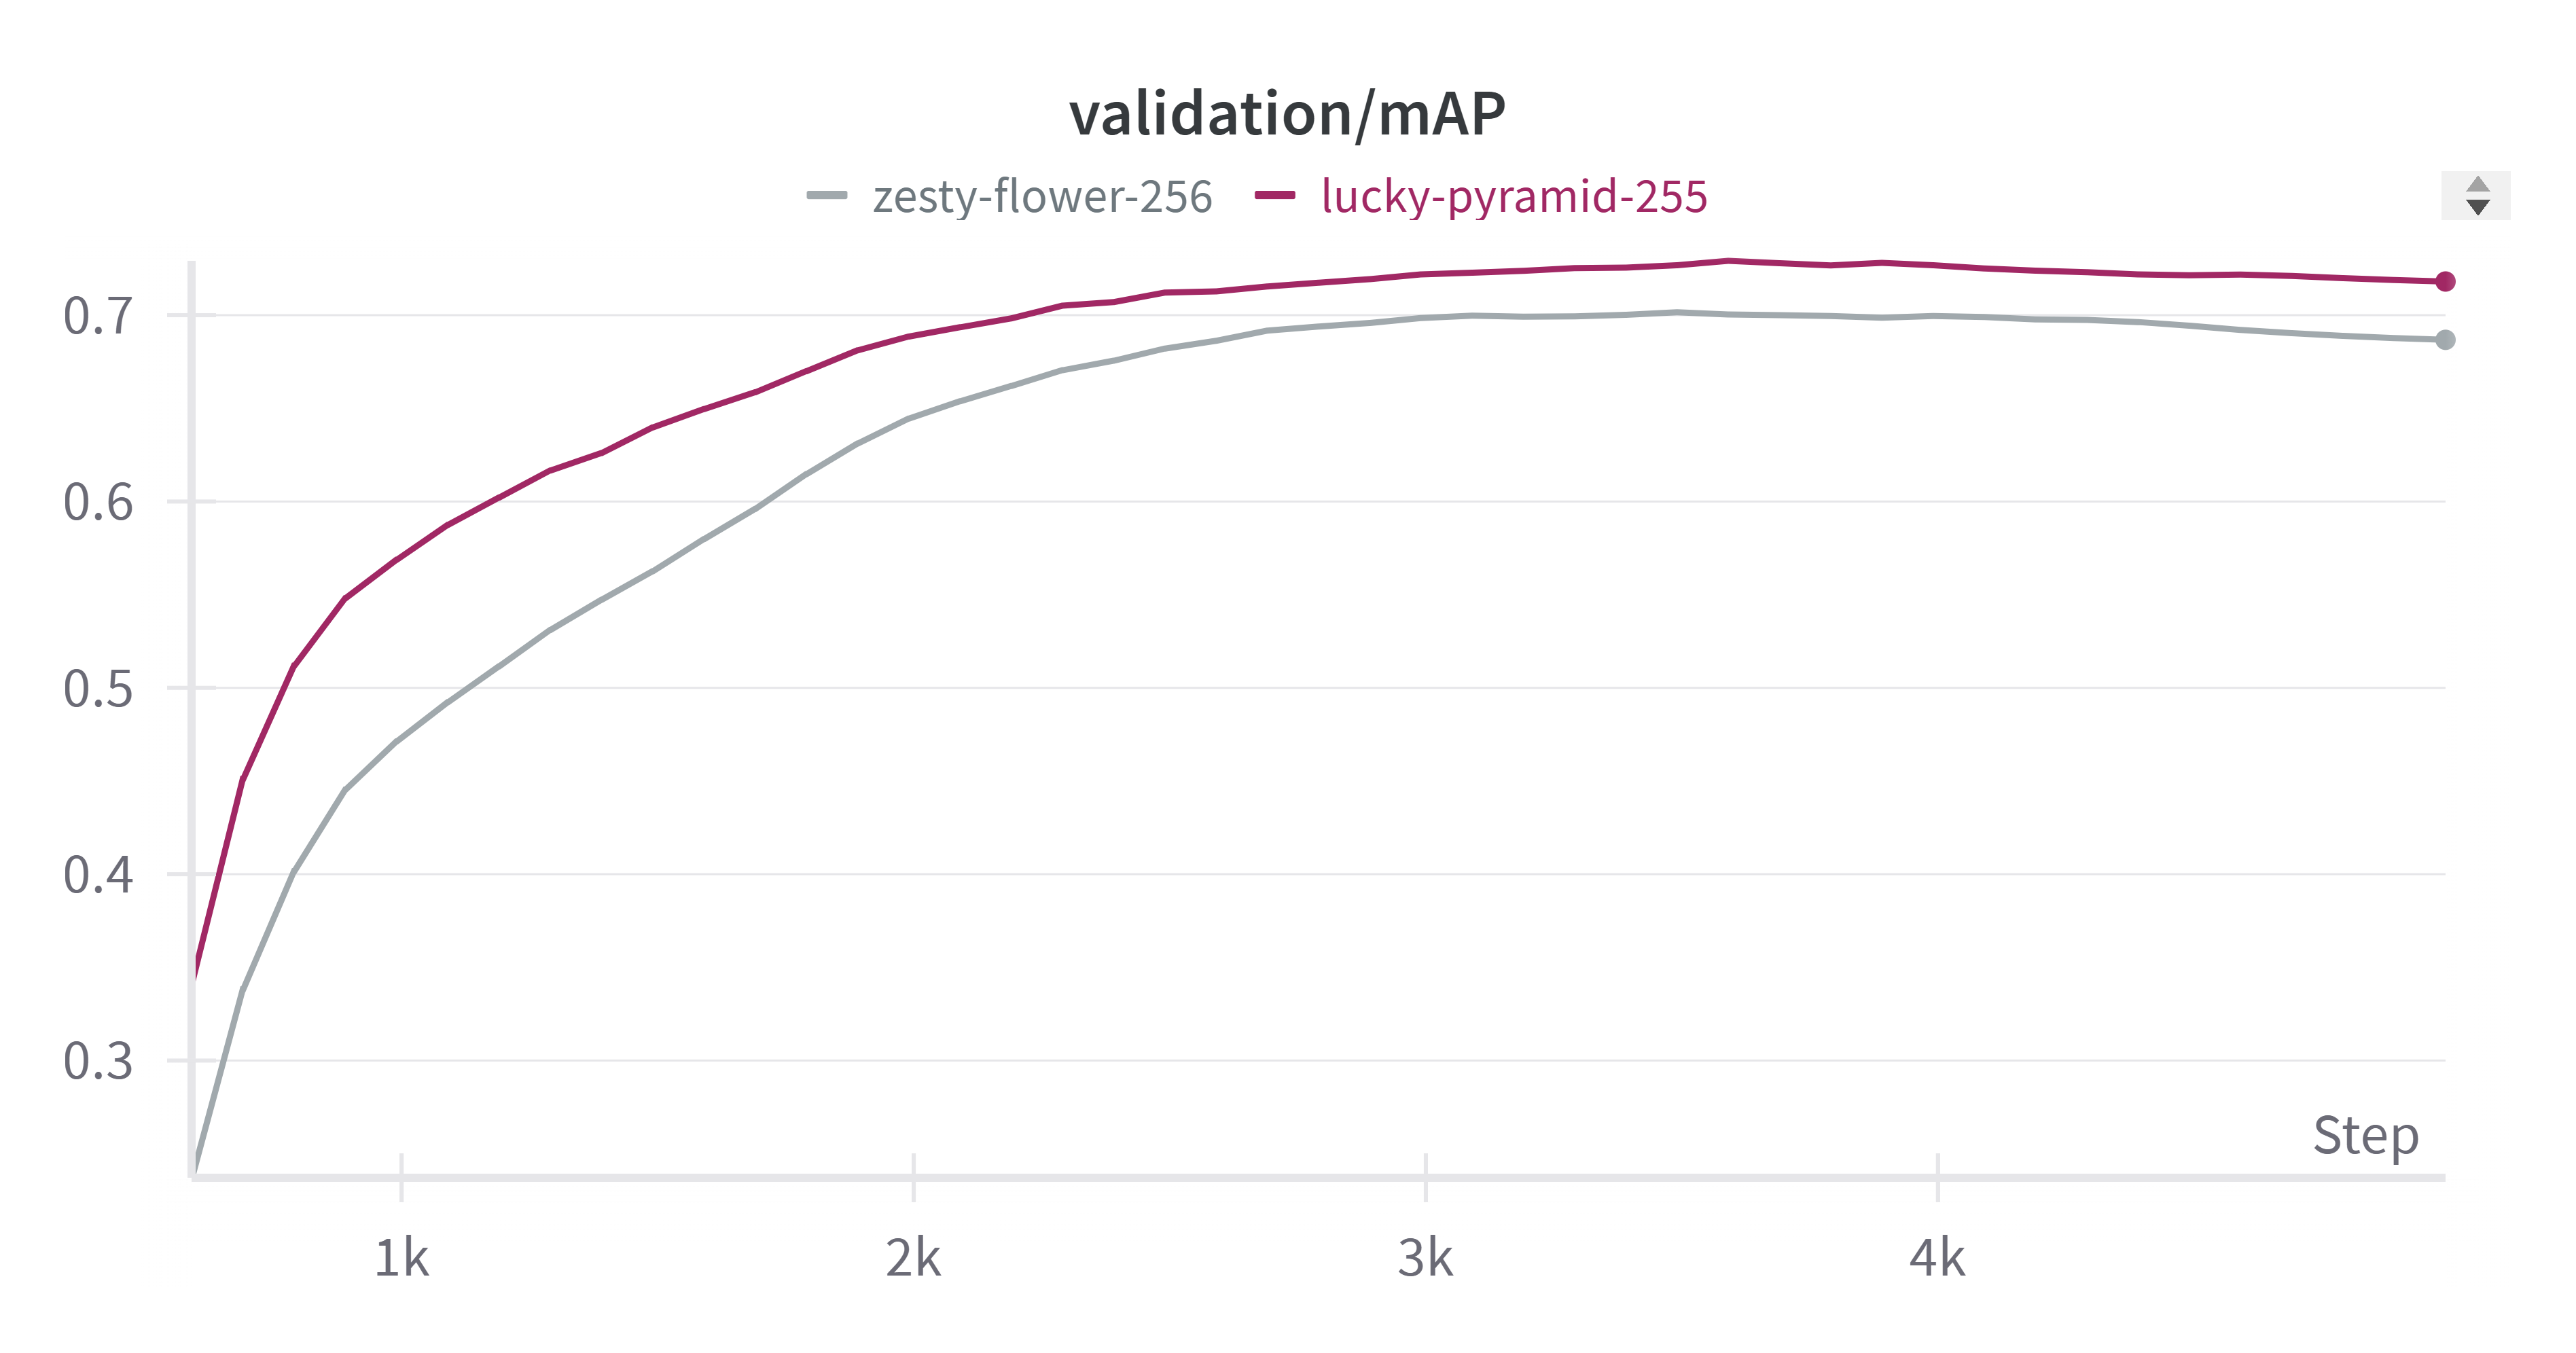
\includegraphics[width=0.75\linewidth]{figures/1408_3200_val.png}
    \caption{Validation per epoch for 3200 features (red) and 1408 features(grey). }
    \label{fig:ex3_val}
\end{figure}
The 1,408-dimensional model achieved a  \acrshort{map} of \(0.686\), while the 3,200-dimensional model reached a \acrshort{map} of \(0.718\) (a 3.2\% absolute gain). Training times were 1 h 15 min and 1 h 23 min respectively, which is an increase of \(\approx11\%\). \autoref{fig:ex3_val} 


\subsection{Discussion}
\label{ssec:ex3_discussion}

blessing of dimensionality. extra important in football or less important. More features => more probable for them to be linearly separable

favorable trade off(in time)

hyperparameters could favor the newer weights

both seem to hit a ceiling at epoch ~32


\section{Experiment 4: Hyperparameter optimization}
\label{sec:experiment4}

The fourth experiment is a hyperparameter optimization experiment.
The goal is to find the best hyperparameters for the \acrshort{vms} model on the SoccerNet dataset.

\subsection{Setup}
\label{ssec:ex4_setup}

\acrlong{wandb} is used to track the hyperparameters and the results for the \acrshort{vms} model trained on SoccerNet-V2 dataset with a 70 \(\%\)-30\(\%\) validation split. All 7 videos of the SoccerNet-V2-format is considered in this approach, including the train, the validation and the testing videos. A Bayesian optimization algorithm is used to find the best importance and correlation of the hyperparameters. The hyperparameters related to the dataset are the only ones modified. Full details about the hyperparameters can be found in \autoref{label:app_sweep}.

A total of 210 runs across three sweeps of 70 runs each were completed. Because of the fast convergence of \acrshort{vms}--models hyperparameter search was an efficient process. 


\subsection{Results}
\label{ssec:ex4_results}

\begin{figure}[ht]
    \centering
    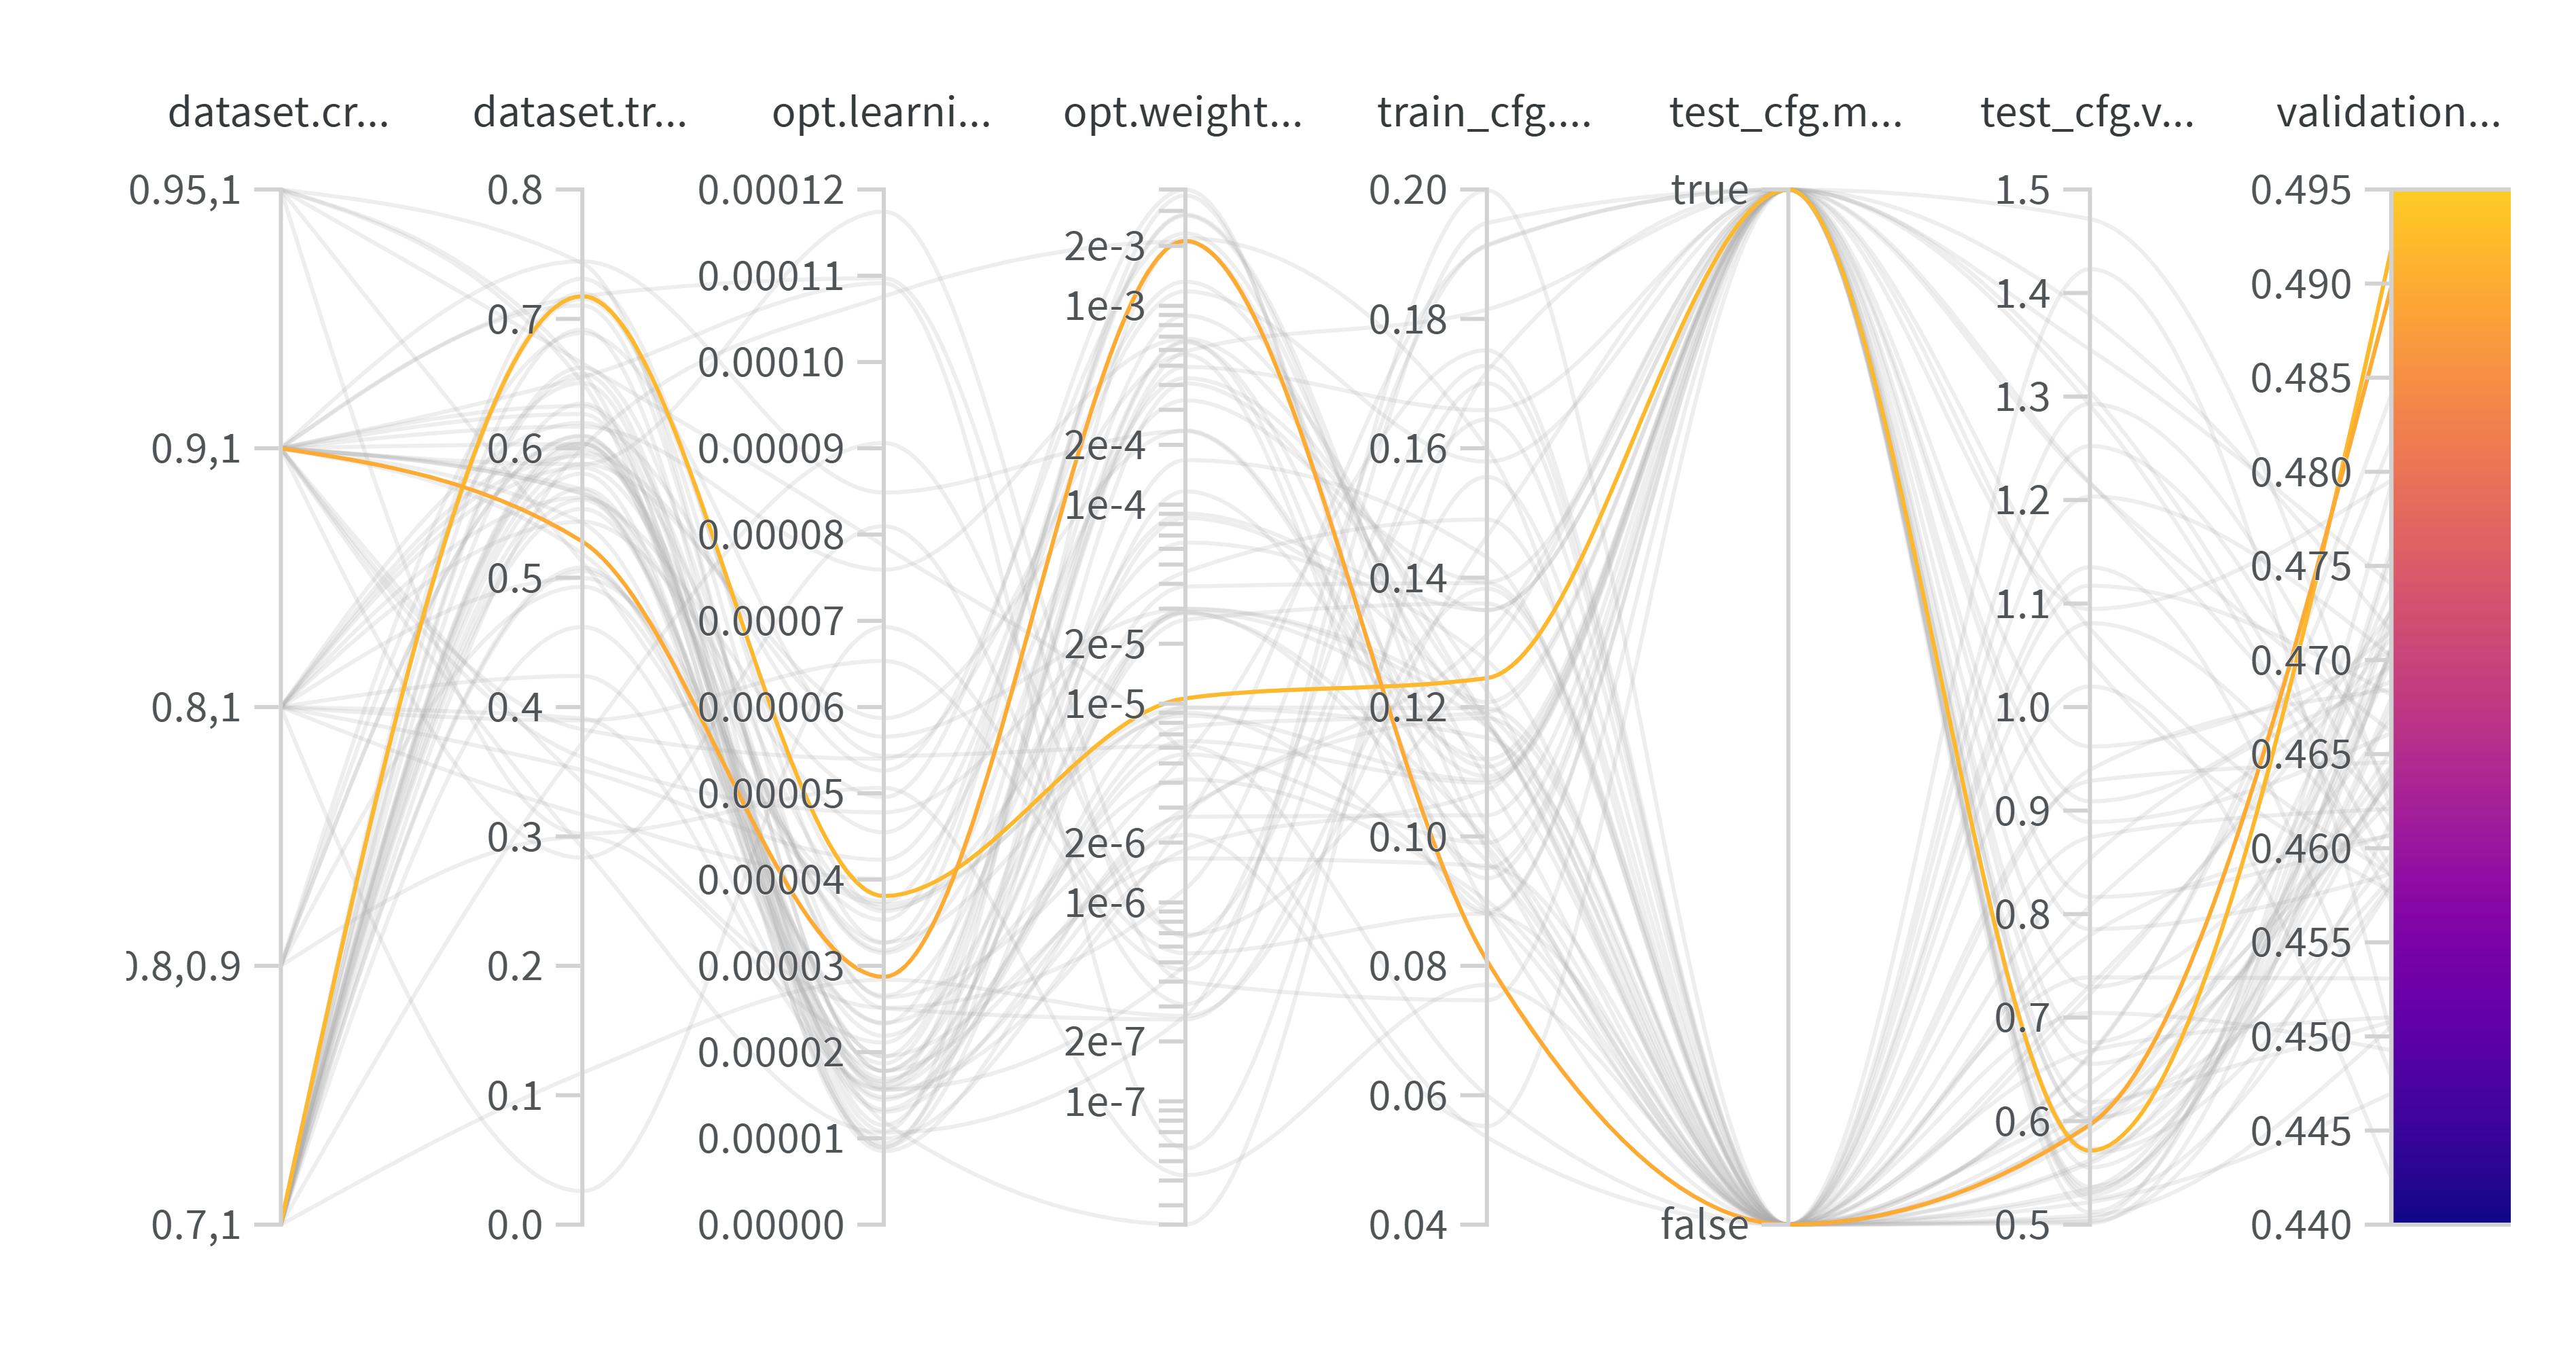
\includegraphics[width=1\linewidth]{figures/sweep_two_best.png}
    \caption{The hyperparameters of the two best results(yellow) compared to all runs (grey) in the thrid sweep. }
    \label{fig:sweep_best_two}
\end{figure}

The sweeps showed a slight improvement to the model. 

Trying to translate the sweep into a single better configration didn't prove useful, but some configurations performed exceptionally better than the rest. But these configurations that worked well, had quite different parameters and was hard to differ. As seen in \autoref{fig:sweep_best_two}, the hyperparameters of the best and second best run in the last sweep differed significantly in their hyperparameters. 

Interpreting the results to create a hyperparameter configuration, as explained in the \autoref{app:sweep_3} the resulting average \acrshort{map} was \(46.77\%\). 

\subsection{Discussion}
\label{ssec:ex4_discussion}

% You found that translating the sweep into a single, consistently better configuration "didn't prove useful," despite some configurations performing "exceptionally better." Why do you believe this was the case?

\begin{figure}
    \centering
    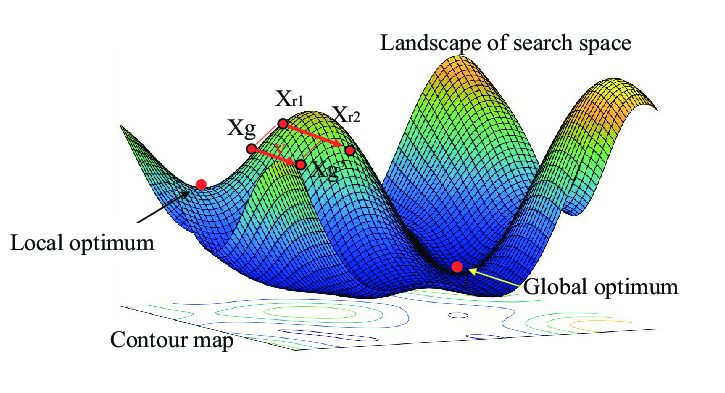
\includegraphics[width=0.75\linewidth]{figures/local_minima.png}
    \caption{A plot of local minima from \cite{fig:multiple_local_minima}. It is not related to any experiments done but its purpose is as a visualization.}
    \label{fig:local_minima}
\end{figure}

It was difficult to translate the sweep into a single consistently better configuration, despite some exceptional outliers. This likely stems from a few different factors. \unsure{multiple local minima, describe in background? bad figure?}

The hyperparameter space might contain multiple local optima. This means there isn't a "peak of performance", but several combinations of hyperparameters cause good results. Picking an average and combining parameters from distinct optima can result in a configuration. For the sake of visualization, look at \autoref{fig:local_minima} and imagine the summits are optima. Picking an average between them will perform worse than individual peaks. 

Hyperparameters often interact in complex and non-linear ways. The success of an \emph{exceptionally better} configuration might depend on a specific interplay between multiple parameters. Changing one parameter in an attempt to generalize or create a "single best" might disrupt this delicate balance, leading to suboptimal performance. The fact that the best two runs had "quite different parameters" (as seen in \autoref{fig:sweep_best_two} supports this idea of different, successful combinations rather than a single clear trend.


% What does the observation that the two best runs in the last sweep had "quite different parameters" (as shown in \autoref{fig:sweep_best_two}) imply about the sensitivity of the \acrshort{vms} model to its hyperparameters on the SoccerNet dataset?
These two runs can imply that there exist multiple good configurations. The interaction between the parameters matters more than the individual values. A specific value for one hyperparameter might work well only in conjunction with others. The two good runs in \autoref{fig:sweep_best_two} could represent two different, good synergies. 

% How does \autoref{fig:sweep_best_two} support your hypothesis of "Multiple local optima in the search space"? What are the broader challenges or implications of such a landscape for hyperparameter tuning?

If the hyperparameter landscape had a single, dominant global optimum, one would expect the best-performing runs to converge towards similar hyperparameter values. The fact that two distinct sets of parameters yield top results suggests that there are at least two separate "peaks" or favorable regions (local optima) in the search space where the model performs exceptionally well. The optimization process has found these different peaks, rather than a single point.

This implies some broader challenges for hyperparameter tuning:

\begin{itemize}
    \item Difficulty in Identifying a Single "Best" Configuration: It becomes hard to declare one set of hyperparameters as universally optimal. What works best might be one of several good combinations.
    \item Increased Search Complexity: Optimization algorithms can easily get "stuck" in a local optimum, potentially missing a better global optimum or other strong local optima. This necessitates more sophisticated search strategies or more extensive random sampling to explore the space adequately.
    \item Sensitivity to Initial Conditions: The starting point of a hyperparameter search can heavily influence which local optimum is discovered.
    \item Challenges in Interpretation: It's harder to draw simple conclusions about the individual impact of each hyperparameter, as their optimal values might be highly dependent on the values of other interacting parameters, leading to different "optimal" combinations.
    \item Reproducibility and Generalization: A specific local optimum found might be very specific to the exact dataset split or even the random seed used during the sweep. Generalizing these findings to slightly different conditions can be more challenging.
    \item 
\end{itemize}


% You noted "something funny is up with the learning rate" and hypothesized a "lower learning rate because football is homogeneous." What specific trends or behaviors in the learning rate did the sweeps reveal to support this? Were there particular ranges that performed better or worse?

As seen in \autoref{app:sweep_3} the best runs in the end shows that the learning rate of the top-performing runs were quite low. The Bayesian search preferred exploring lower learning rates, and especially the thrid sweep showed low learning rates performed best. In the last sweep, learning rate had the highest importance and highest absolute correlation. The correlation was negative. 

Homogeneous data like football actions, where events can be visually similar, a lower learning rate allows the model to make finer adjustments. This can help it learn the subtle distinguishing features without overshooting the optimal weight configurations in the loss landscape, leading to better discrimination between closely related actions.

% You decided to "only tune dataset variables." Which specific variables were these? Based on the 210 runs, which of these dataset-specific hyperparameters appeared to have the most significant impact on performance, and which seemed less critical?

The hyperparameters that were tuned are:
\begin{itemize}
    \item learning\_rate
    \item weight\_decay
    \item drop\_path 
    \item batch\_size (explored in Sweep 1, then fixed)
    \item voting\_thresh
    \item trunc\_thresh
    \item crop\_ratio (introduced in Sweep 3)
    \item multiclass\_nms (evaluated in Sweep 3)
    \item max\_seq\_len (explored initially, then ignored)
    \item pre\_nms\_topk (explored initially, then ignored)
    \item clip\_grad\_l2norm (explored initially, then ignored)
    \item 
\end{itemize}

\textbf{Learning rate} appeared to be the most significant value. While its correlation varied, Sweep 3 indicated that the best performance was concentrated in a very specific low range (around 0.00003-0.00004). 

\textbf{Crop ratio} showed clear performance differences between its settings. As the data augmentation parameter, it was expected to have a higher impact than it did. 

\textbf{droppath} was the most important with the least correlation in the first sweep. It was tuned in Sweep 2 and selected as a fixed value for Sweep 3. 

Sweep 1 deemed \textbf{batchsize} to be unimportant. Ideal values were found for voting\_thresh and trunc\_thresh in Sweep 3. 

% Were there any other hyperparameters (or ranges) that consistently led to better or worse results, or any notable interactions between parameters observed from the wandb logs?

% The interpreted configuration resulted in an average \acrshort{map} of (46.77\%). How does this compare to your baseline \acrshort{vms} performance in Experiment 1 (e.g., 45.99\%)? The default parameters provided an average map of 48.73\%. The best run in the sweep had 49.18\% Is this improvement practically significant?

The interpreted sweep configuration achieved an average \acrshort{map} of $46.77\%$. Default parameters on the same dataset got $48.73\%$ average \acrshort{map}. This is a significant decrease in performance of almost $2\%$. When comparing on the same data split (70\%/30\% using all 7 videos), the default hyperparameters outperformed the configuration derived from interpreting the sweep results. This suggests that the process of creating a single "interpreted" set of hyperparameters was not successful in finding a configuration superior to the defaults for this specific dataset setup.

The best run in the sweep got a $49.18\%$ average \acrshort{map}. That is $2.41\%$ higher than the interpretation and $0.45\%$ higher than the default parameters. It identifies that the sweep identified some configurations that outperformed the default, but an interpreted result did not exist. 


% You suspect "negative/neutral results" might be because "features are trained to match the preprocessing timeline." Could you elaborate on this? How might the pre-trained nature of the features interact with the dataset-specific hyperparameters you were tuning?

The features from \acrshort{vmae} are implicitly optimized to represent video information based on the original preprocessing pipeline. The ability to improve performance could be limited if the features are "happiest" when processed in a way that mirrors the feature extraction. It could be that the dataset hyperparameters are tuned to the features structure, not the features content, to some extent. The tuning might then be exploring variations that don't fundamentally alter or improve upon the information already captured by the features. \unsure{it makes sense to me, but is a bit hard to read. i mean to tell that parameters fit preprocessing and not soccer data}

% Could the modest overall improvement also suggest that the default hyperparameters for \acrshort{vms} are already reasonably well-optimized for this task, or that the search space explored didn't contain dramatically better configurations?

results indicate that while minor gains are possible through extensive tuning, the default \acrshort{vms} hyperparameters seem to be a very effective starting point for the SoccerNet dataset. The hyperparameter space explored, while yielding some improvements, did not reveal overwhelmingly superior configurations.

% What specific evidence from the sweeps led to the concern about "overfit on 30 percent validation"? For instance, how did the training loss/metrics compare to validation loss/metrics for high-performing runs versus others?

\begin{figure}
    \centering
    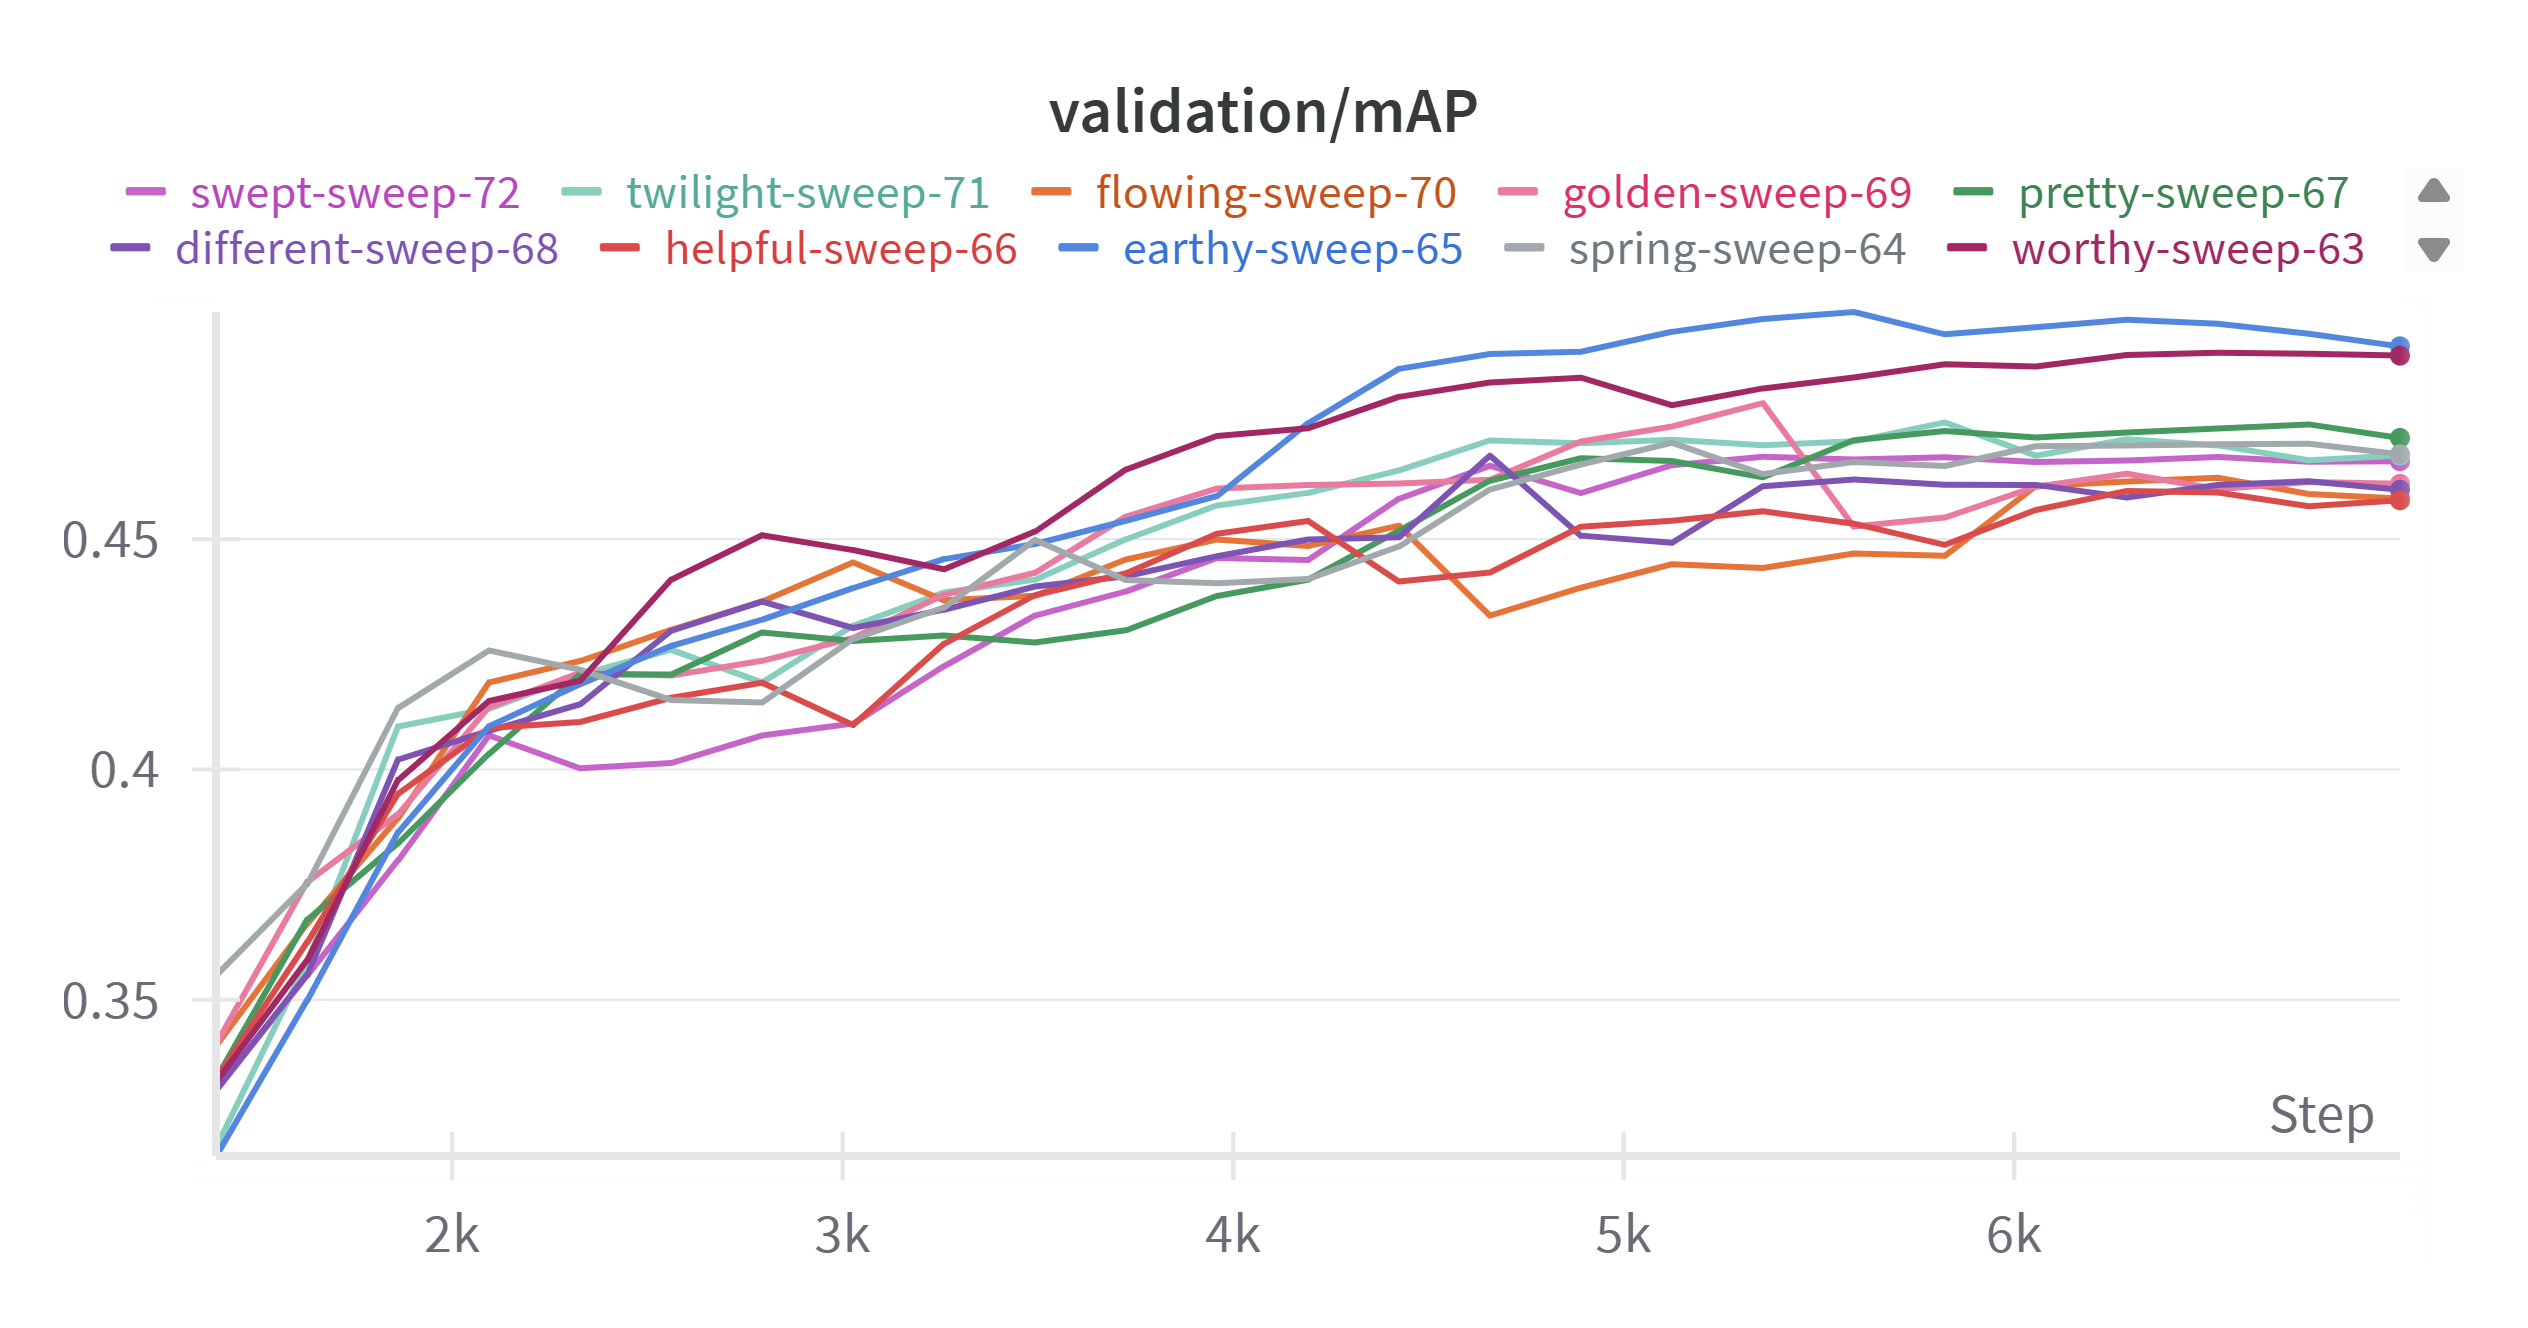
\includegraphics[width=0.75\linewidth]{figures/plateu_sweep.png}
    \caption{Validation plotted against steps for the latest runs in Sweep 3. }
    \label{fig:plateu_sweep}
\end{figure}
\begin{figure}
    \centering
    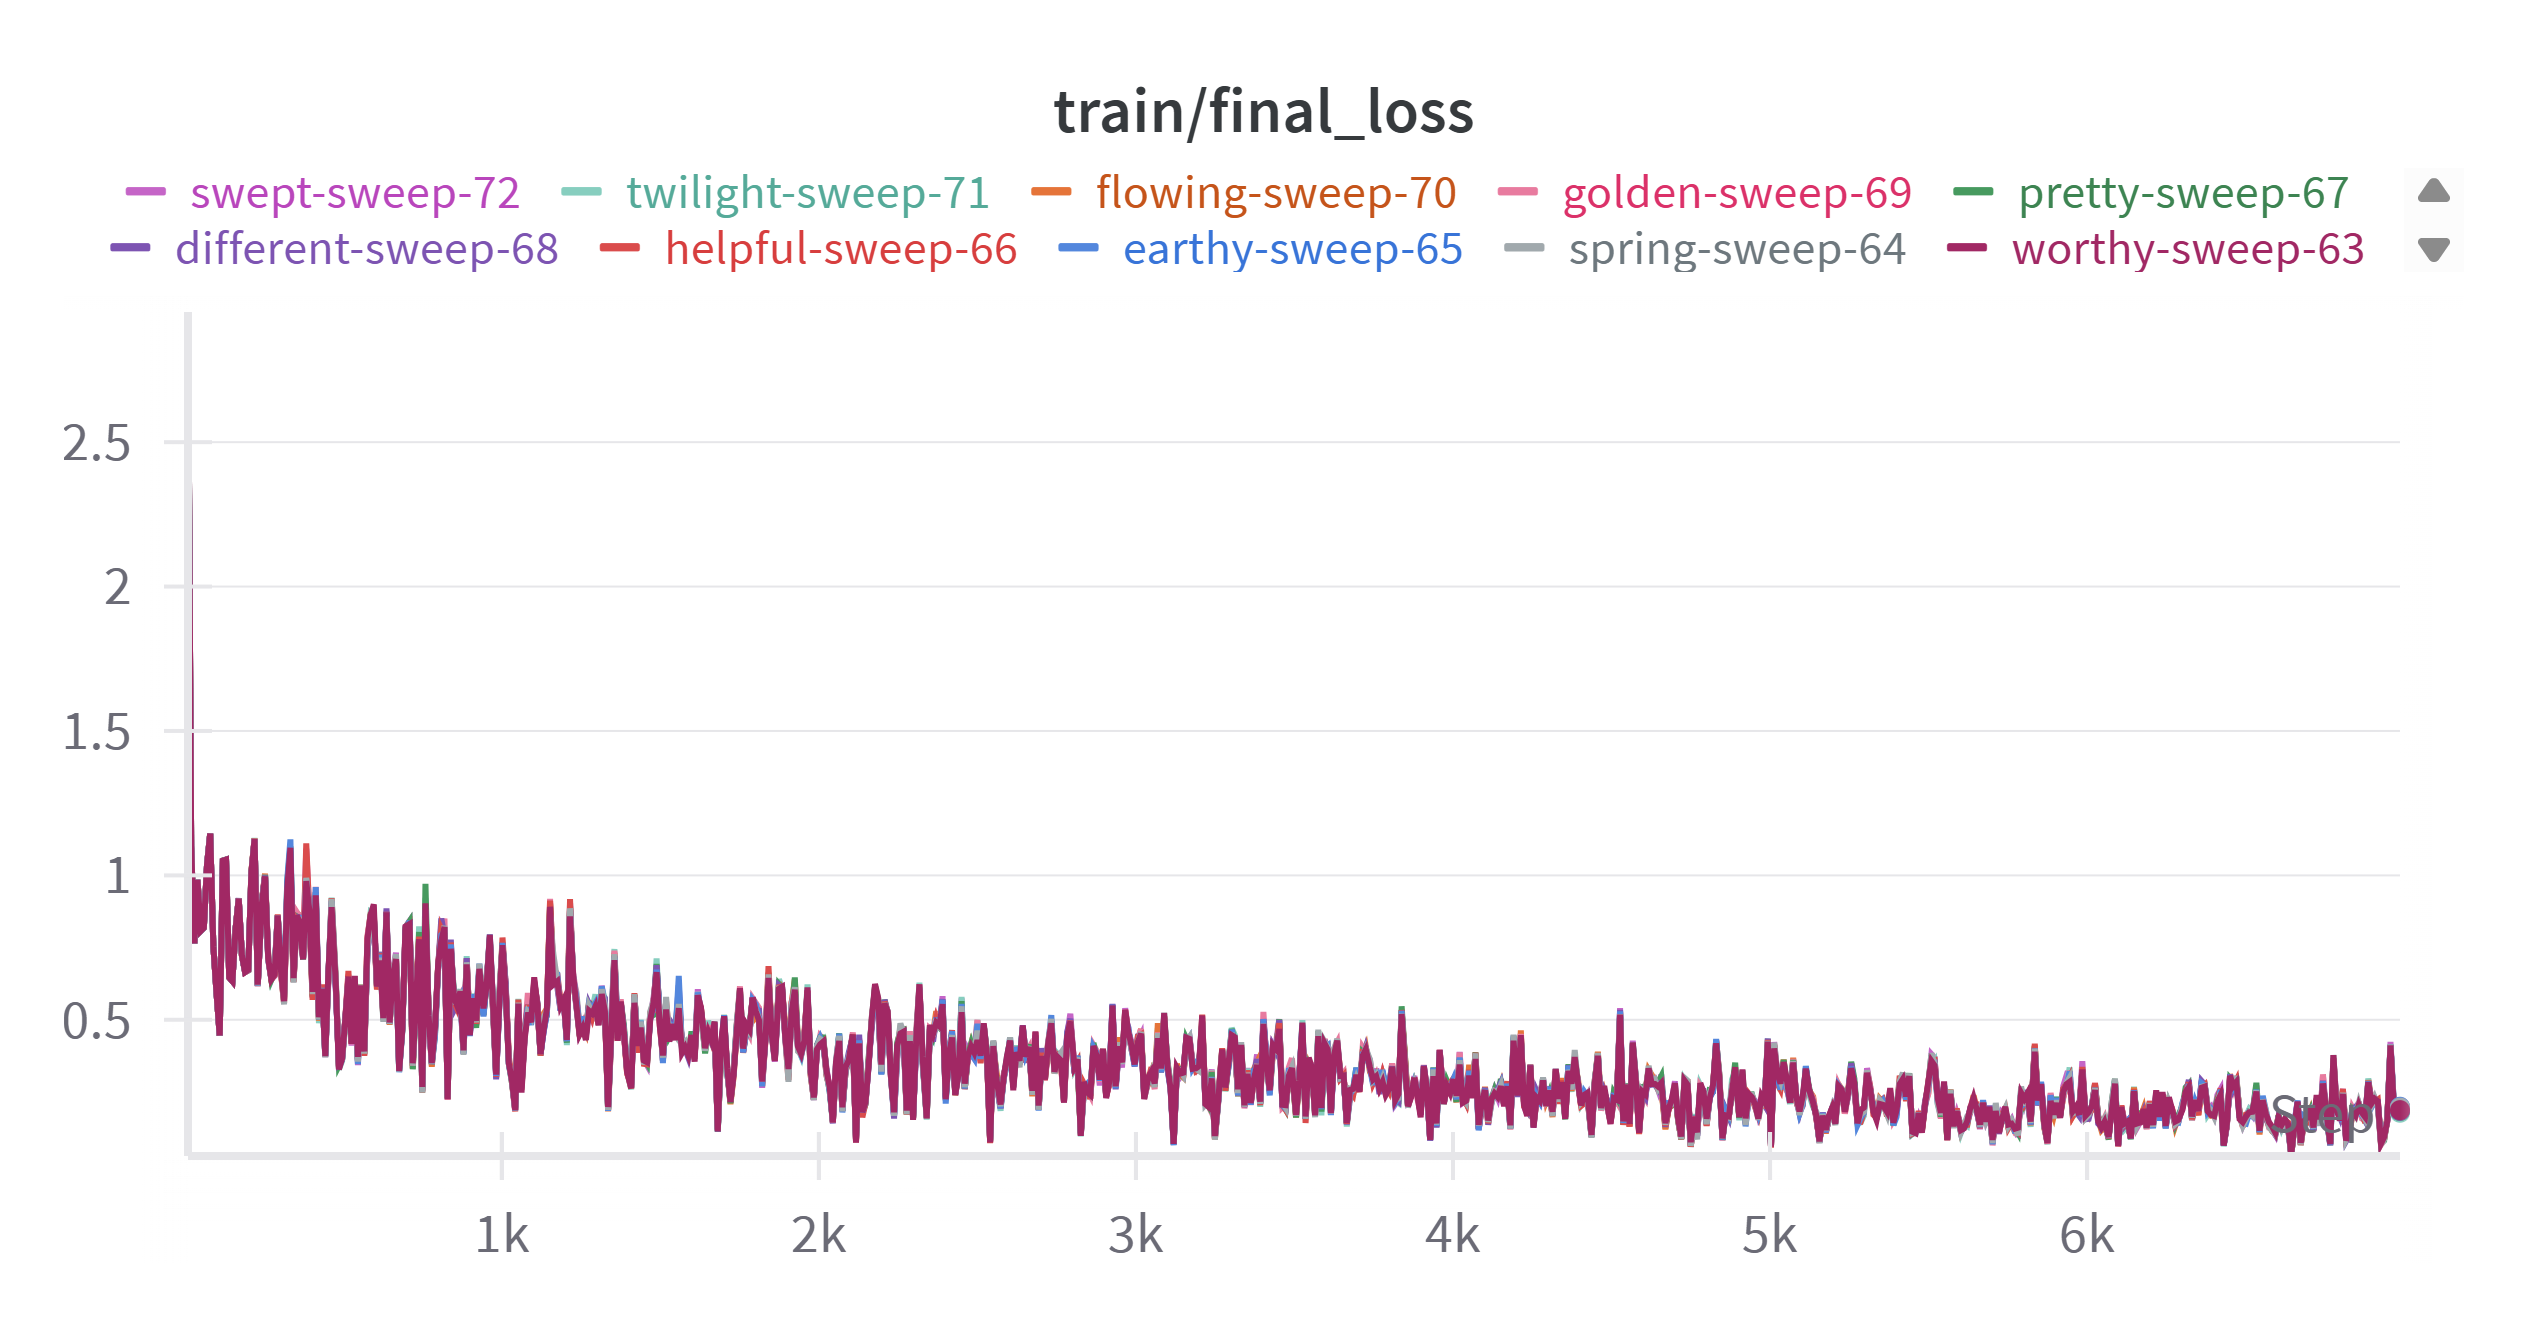
\includegraphics[width=0.75\linewidth]{figures/plateu_loss.png}
    \caption{Training loss plotted against steps for the latest runs in Sweep 3.}
    \label{fig:plateu_loss}
\end{figure}
The general trend of the sweep was for the runs to plateau relatively early, as seen in \autoref{fig:plateu_sweep}. At the same time, the loss was relatively low and stable. This indicates the model stops generalizing to validation data and fits to noise in training data.

% Why was a Bayesian optimization algorithm chosen? Given your findings (e.g., multiple local optima), do you believe this was the most suitable approach, or might other methods (like random search, or a more targeted search after initial exploration) have been beneficial?

Bayesian optimization aims to find the best hyperparameters in fewer iterations. The algorithm is suited for a landscape with multiple optima, because there is no inherent assumption of a single optimum. As seen in the Sweeps it found some exceptionally good runs compared to the average. 

Random search is effective for initial exploration. It has a use case if the initial parameters are considered to be close to a local optima which is not the global. I had no reason to believe this, neither the motivation of exploring enough variables compared to the original authors\cite{li_videomamba_2024}.

% Were the 210 runs across three sweeps sufficient to thoroughly explore the hyperparameter space, or do you feel more runs could have yielded further insights?

It might have been beneficial to start with a more extensive exploration before running the Bayesian search. This would require a lot more than the 210 runs, on \acrshort{idun} which was already under pressure. I find it probable that the default parameters, which are second \acrshort{sota} on the THUMOS benchmark, are close to the global optima. For sustainability both with regards to power usage but also fair usage of the computational resources, I think it is correct to not continue the search. If the results showed a greater increase, it the decision must be reconsidered.

% Despite the difficulty in pinpointing a single "best" configuration, what practical advice or general heuristics for tuning \acrshort{vms} on SoccerNet-like datasets can be derived from your 210 runs?


% How do the outcomes of this hyperparameter optimization experiment influence your confidence in, or interpretation of, the results from Experiment 1 (accuracy comparison)?

This experiment increases my confidence in the results of Experiment 1. The experiment proves that the default hyperparameters performs well. The sweeps only provided a slight increase in accuracy, and its interpretation performed worse. It proves the performance reported in Experiment 1 is a fair representation.

Experiment 1 mentioned that \textit{Using default hyperparameters from their original papers might not be optimal for the specific SoccerNet-V2 dataset... potentially disadvantaging one or both models.}\autoref{ssec:ex1_discussion}. Experiment 4 explored this for \acrshort{vms} and found its defaults were already strong. However, \acrshort{tdeed} was not subjected to a similar hyperparameter optimization. Therefore, while there is more confidence that \acrshort{vms}'s default performance is close to its tuned potential on this dataset, the same cannot be said for \acrshort{tdeed}. \acrshort{tdeed} might still have untapped potential if its hyperparameters were similarly optimized for SoccerNet.


% What are the key lessons learned from this experiment that will inform subsequent experiments or the final conclusions of your thesis?

To conclude:
\begin{itemize}
    \item \textbf{Default Hyperparameters are Robust}: The default hyperparameters for \acrshort{vms} provide a strong baseline. Extensive tuning might only yield marginal gains, suggesting that the original authors provided well-chosen defaults. This implies that for future comparisons or new experiments, starting with defaults is a reasonable approach, and significant deviations in performance are more likely due to other factors (model architecture, data, etc.) than suboptimal default settings.
    \item \textbf{Hyperparameter Optimization is Complex and Not Always a Silver Bullet}: The search space can have multiple local optima, making it difficult to find a single, universally "best" configuration. Trying to create an "interpreted" best configuration from a sweep might not outperform the defaults or the best individual run found. This cautions against over-reliance on hyperparameter sweeps to unlock performance gains if a model is already well-designed.
    \item \textbf{Learning Rate is a Key Lever, Especially for Homogeneous Data}: For datasets like SoccerNet, where actions can be visually similar, a lower learning rate appears beneficial. This is a concrete takeaway for tuning \acrshort{vms} on such data.
    \item \textbf{Pre-trained Features Influence Tuning}: The characteristics of pre-trained input features can constrain the effectiveness of tuning downstream hyperparameters. The features might already be optimized for a certain processing "timeline," limiting how much dataset-specific tuning can improve things.
    \item \textbf{Resource Constraints and Practicality}: Exhaustive hyperparameter search is computationally expensive. The decision to stop searching needs to be balanced against the potential for gains and available resources, especially if initial results (like strong default performance) suggest diminishing returns.
    \item \textbf{Impact on Comparative Experiments}: The finding that \acrshort{vms} defaults are strong lends more credibility to comparisons made using these defaults (like in Experiment 1). However, it also highlights that if a competing model wasn't similarly tuned, the comparison might not fully reflect its potential.
    \item \textbf{Focus on Broader Factors}: Given the modest gains from hyperparameter tuning, other factors like feature quality (Experiment 3), model architecture, data augmentation, and post-processing strategies might offer more significant avenues for performance improvement.
\end{itemize}


\section{Experiment 5: T-DEED with and without joint training}
\subsection{Setup}
\label{ssec:ex5_setup}
\begin{figure}
    \centering
    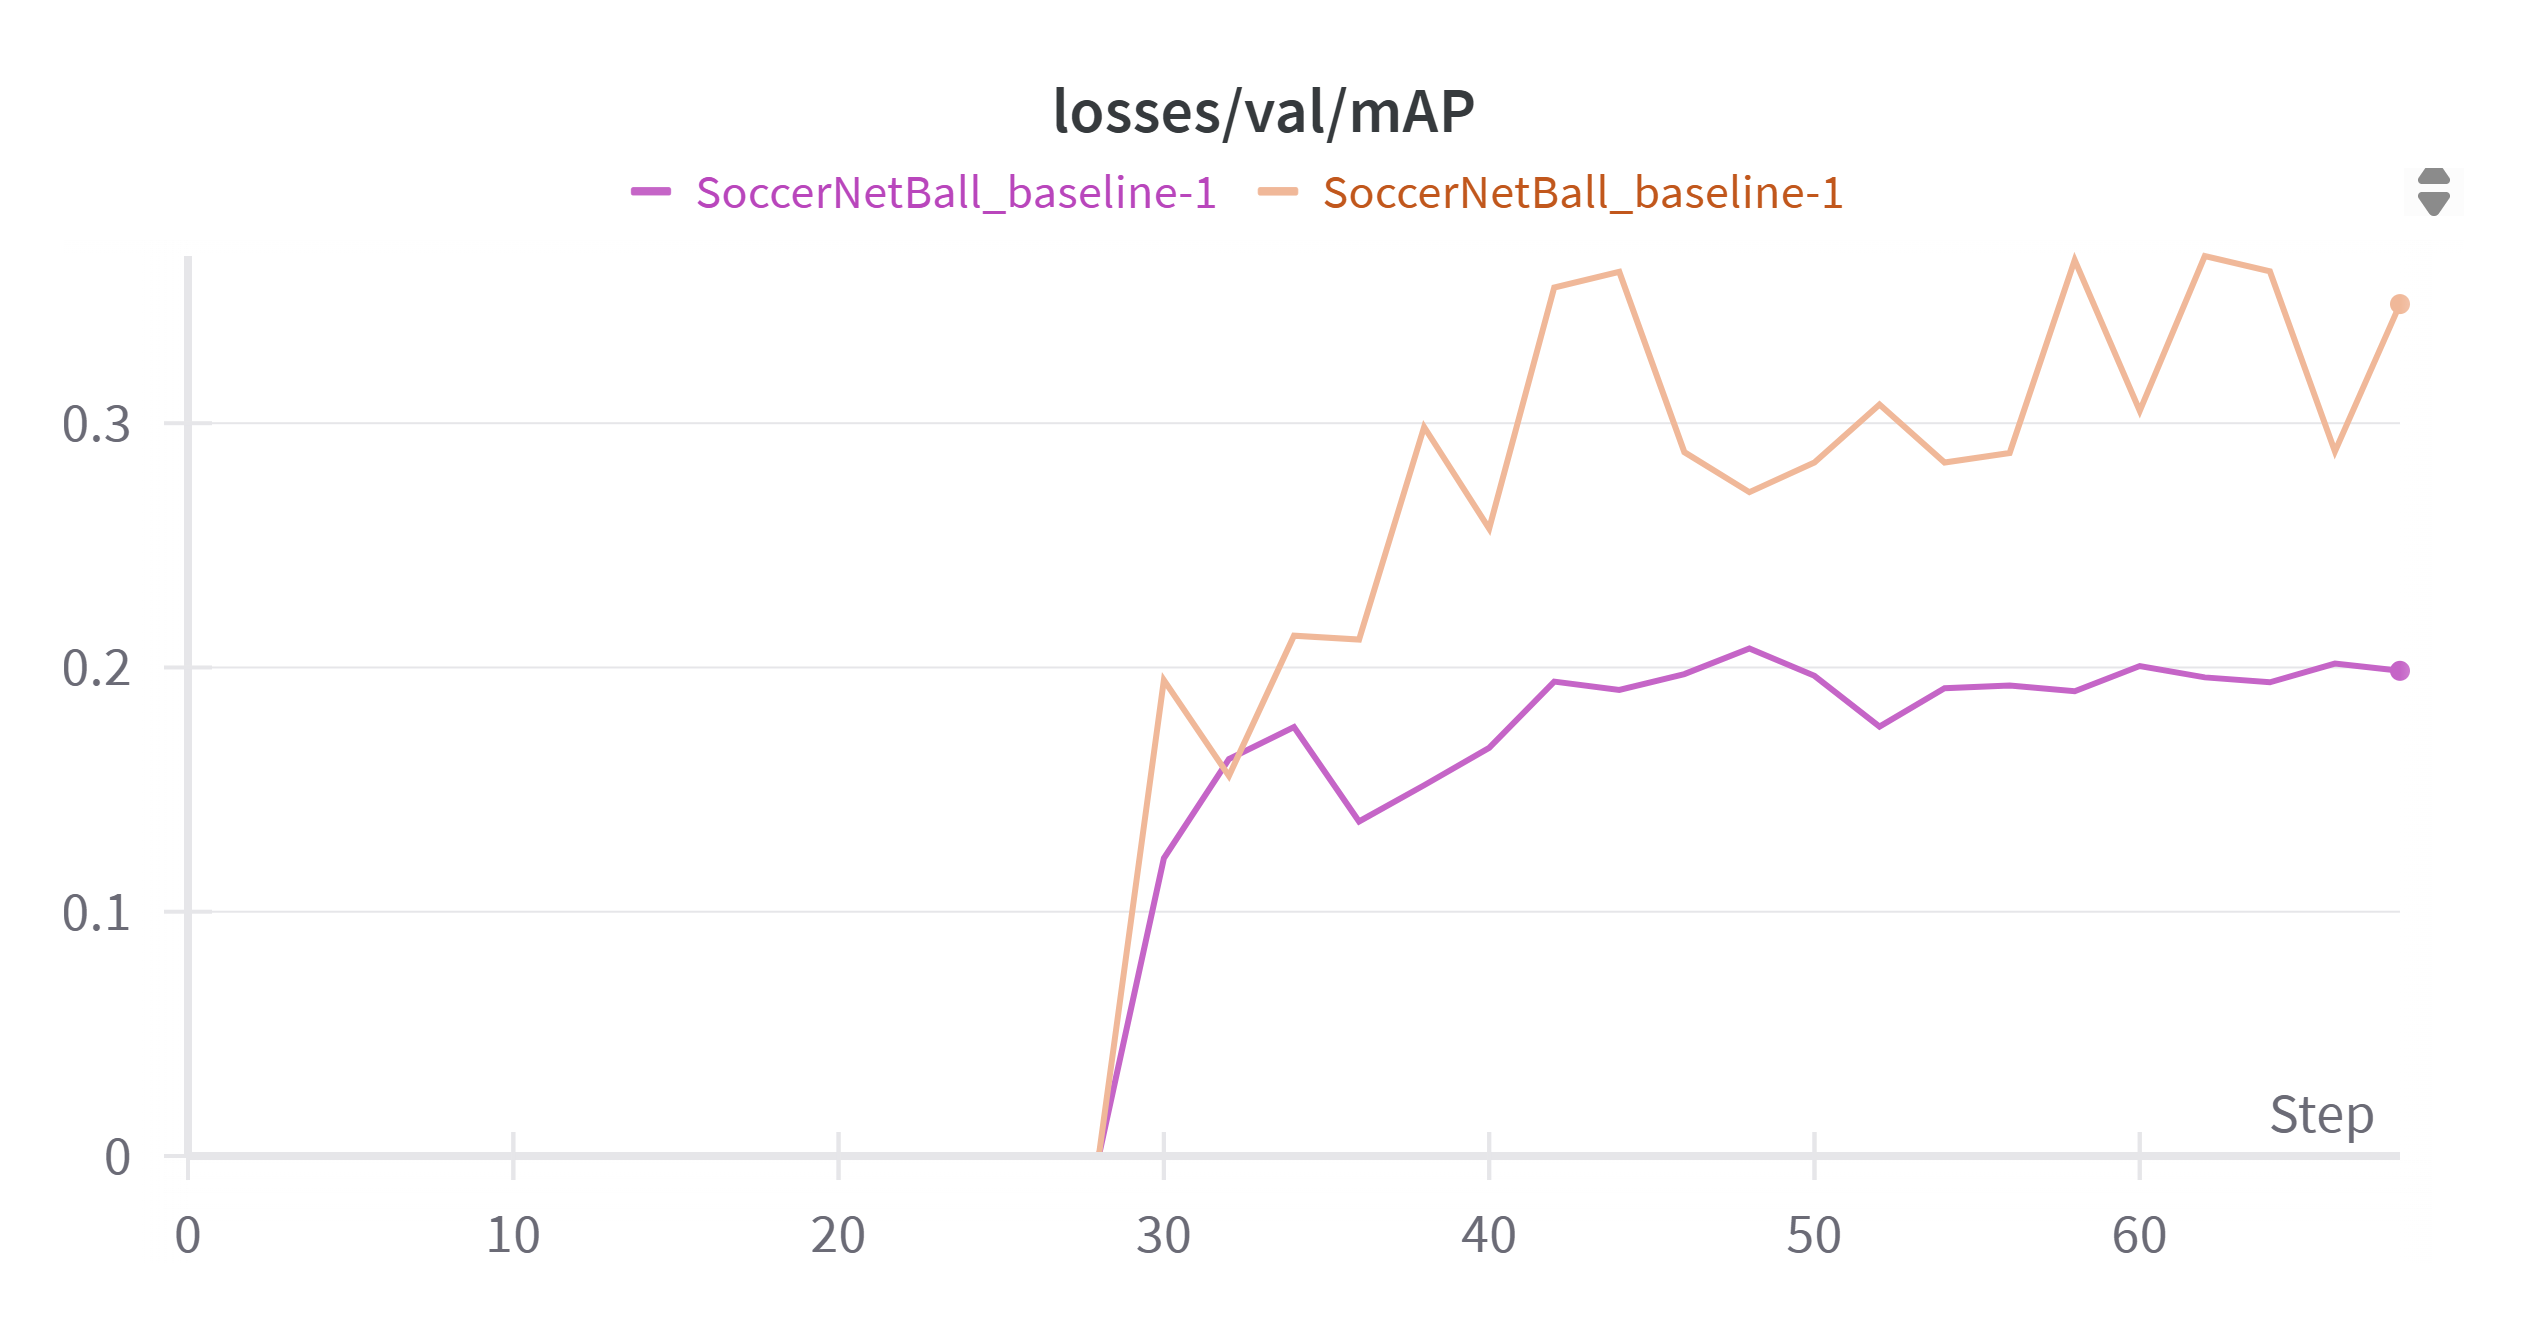
\includegraphics[width=0.75\linewidth]{figures/500_7_val_compare.png}
    \caption{Validation per epoch for the model trained with joint training (507 videos) in brown and the model trained without joint training (purple).}
    \label{fig:500_7_val_compare}
\end{figure}


\subsection{Results}
\label{ssec:ex5_results}


another experiment where I just run array jobs with different train/val splits

\subsection{Discussion}
\label{ssec:ex5_discussion}


\section{Summary}
vms runs on any GPU, but tdeed needs a lot of memory and only runs on premium GPUs.